\documentclass[margin=2mm]{standalone}
\usepackage{tikz}
\usetikzlibrary{fit}

\begin{document}
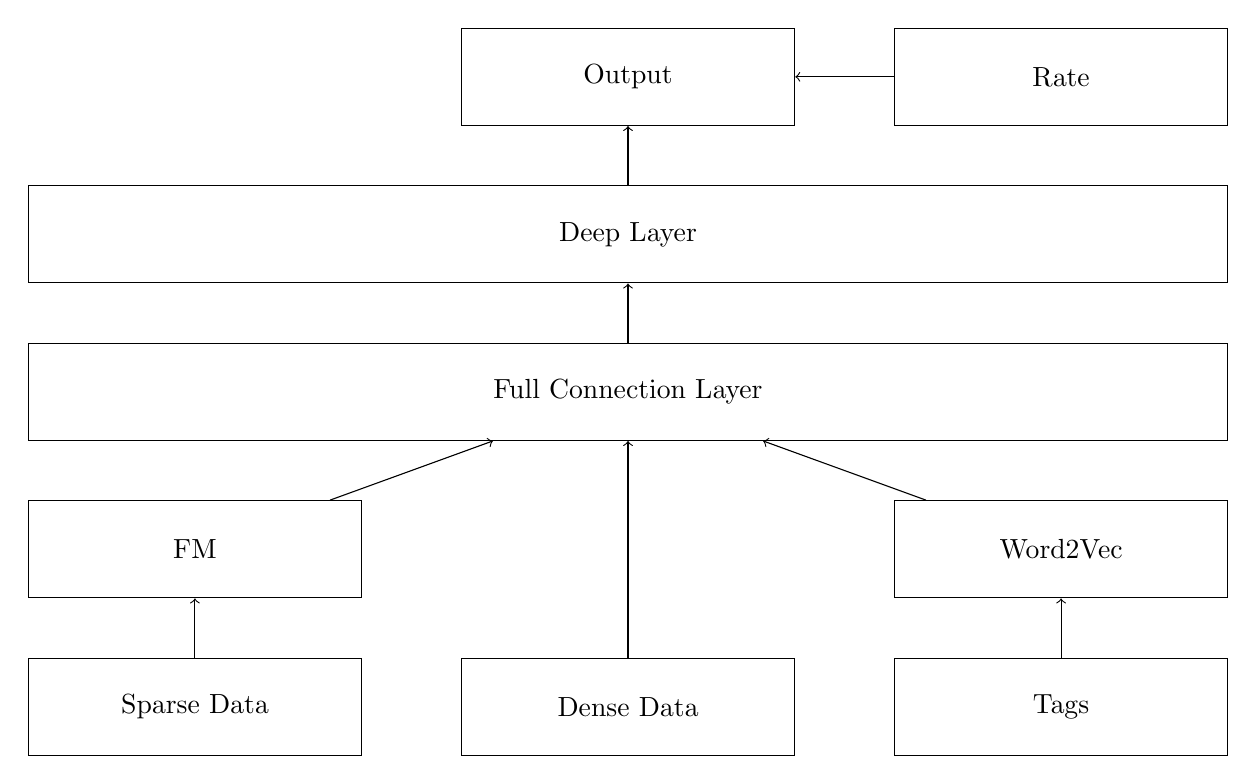
\begin{tikzpicture}
    \node[draw, fit={(0,0) (4,1)}, label=center:{Sparse Data}] (sd) {};
    \node[draw, fit={(5.5,0) (9.5,1)}, label=center:{Dense Data}] (dd) {};
    \node[draw, fit={(11,0) (15,1)}, label=center:{Tags}] (tags) {};

    \node[draw, fit={(0,2) (4,3)}, label=center:{FM}] (fm) {};
    \node[draw, fit={(11,2) (15,3)}, label=center:{Word2Vec}] (w2c) {};

    \node[draw, fit={(0,4) (15,5)}, label=center:{Full Connection Layer}] (ed) {};
    \node[draw, fit={(0,6) (15,7)}, label=center:{Deep Layer}] (dl) {};

    \node[draw, fit={(5.5,8) (9.5,9)}, label=center:{Output}] (o) {};
    \node[draw, fit={(11,8) (15,9)}, label=center:{Rate}] (rate) {};

    \draw[->] (sd) -- (fm);
    \draw[->] (tags) -- (w2c);
    \draw[->] (fm) -- (ed);
    \draw[->] (dd) -- (ed);
    \draw[->] (w2c) -- (ed);
    \draw[->] (ed) -- (dl);
    \draw[->] (dl) -- (o);
    \draw[->] (rate) -- (o);
\end{tikzpicture}
\end{document}